% !TEX encoding = UTF-8
% !TEX TS-program = pdflatex
% !TEX root = ../tesi.tex

%**************************************************************
\chapter{Pulumi, an IaC platform}
\label{cap:introduction-pulumi}
%**************************************************************

\intro{An introduction to Pulumi, to its advantages and its core functioning}\\

%**************************************************************
\section{Introduction to Pulumi}
Pulumi is a cloud engineering platform that enables developers and infrastructure teams to build, deploy, and manage cloud-native applications and infrastructure across multiple cloud providers, including AWS, Azure, Google Cloud, and Kubernetes.\\
Pulumi provides a programming model that allows developers to use familiar languages, such as Python, JavaScript, TypeScript, Go, and (partially) Java to define their IaC and manage it as software.
In fact, it belongs to the second generation tools of the IaC.\\
As already mentioned in the \hyperref[cap:introduction-to-iac]{Introduction to Infrastructure as Code} chapter, such an approach, makes it easier to automate the deployment and management of infrastructure and applications, as well as to collaborate across teams and projects.\\
Pulumi is innovative because, differently from most of all the other second generation IaC tools, has been able to abstract the problem of having many different cloud providers, and also of really different natures (such as Kubernetes vs AWS), while supporting many general purpose languages at the same time.
Its solution is letting the user rely on a single IaC platform to manage any kind of resource on any cloud provider.
Potentially, Pulumi could support any technolgy that is showing \gls{REST API}s.
This feature is making Pulumi an innovative IaC platform that rise IaC on a new level.\\
Pulumi offers a range of tools and features to simplify the development and management of cloud infrastructure, including version control, testing, monitoring, and security.
It also provides templates, examples, and libraries for common infrastructure patterns and services, such as containers, serverless functions, databases, and networking.\\
Overall, Pulumi aims to streamline the process of building and managing modern cloud-native applications and infrastructure, while providing a flexible and developer-friendly experience.

\subsection{The great advantages of Pulumi as a second generation IaC tool}
First of all, as mentioned in the \hyperref[sssec:second-wave]{Serverless Infrastructure as programming language code - the second wave} paragraph, all the functionalities that comes along a programming language are letting us achieve more robust and powerful solutions for our infrastructure, rather than what we could achieve with the expressive power of a markup language (like the one used with \gls{Terraform}).\\
%Being the focus of this thesis, we'll discuss more about such advantages in the \hyperref[cap:comparisons]{Comparison between the languages for Pulumi and the advantages of Scala} chapter.\\
Furthermore, as aforementioned, Pulumi is a multi-cloud tool. Thanks to this we can rely on a single IaC tool for managing resources across different cloud platforms.\\
Moreover, Pulumi lets the user choose its favorite programming language, or the one that in its opinion is a best-fit for the need to be addressed.
In other words, such a choice can both reduce the requirements placed on the user's knowledge, since it can choose among many different programming languages, 
and at the same time offer different programming paradigms to choose from, so that for any need there is a programming language that is addressing such a need better than the others.\\
Finally, Pulumi comes with a range of integrated tools and features, such as automatic parallelism, drift detection, and \textit{stack} references, making it easier to manage complex infrastructure and deployments.

\section{Pulumi functioning}
\label{sec:pulumi-functioning}

\subsection{Overview of the functioning}
Pulumi functioning is based on the interoperation of three main parts:
\begin{description}
  \item[Source code] is used to declare the resources to be created on the respective cloud service provider
  \item[Backend engine] such engine could run on the Pulumi server or locally on the machine. When the \texttt{pulumi up} command is executed, a state file is created and stored in the backend engine. Such a file is representing a "screenshot" of the resources declared in the user's project. The engine then uses such a file to create the descripted resources on the cloud providers, thanks to the REST APIs that they are exposing
  \item[Resources of the providers] are the actual resources on the cloud providers
\end{description}
This image, taken from the official site of \href{https://www.pulumi.com/docs/intro/concepts/how-pulumi-works/}{Pulumi}, is representing the aforementioned architecture.
\begin{center}
  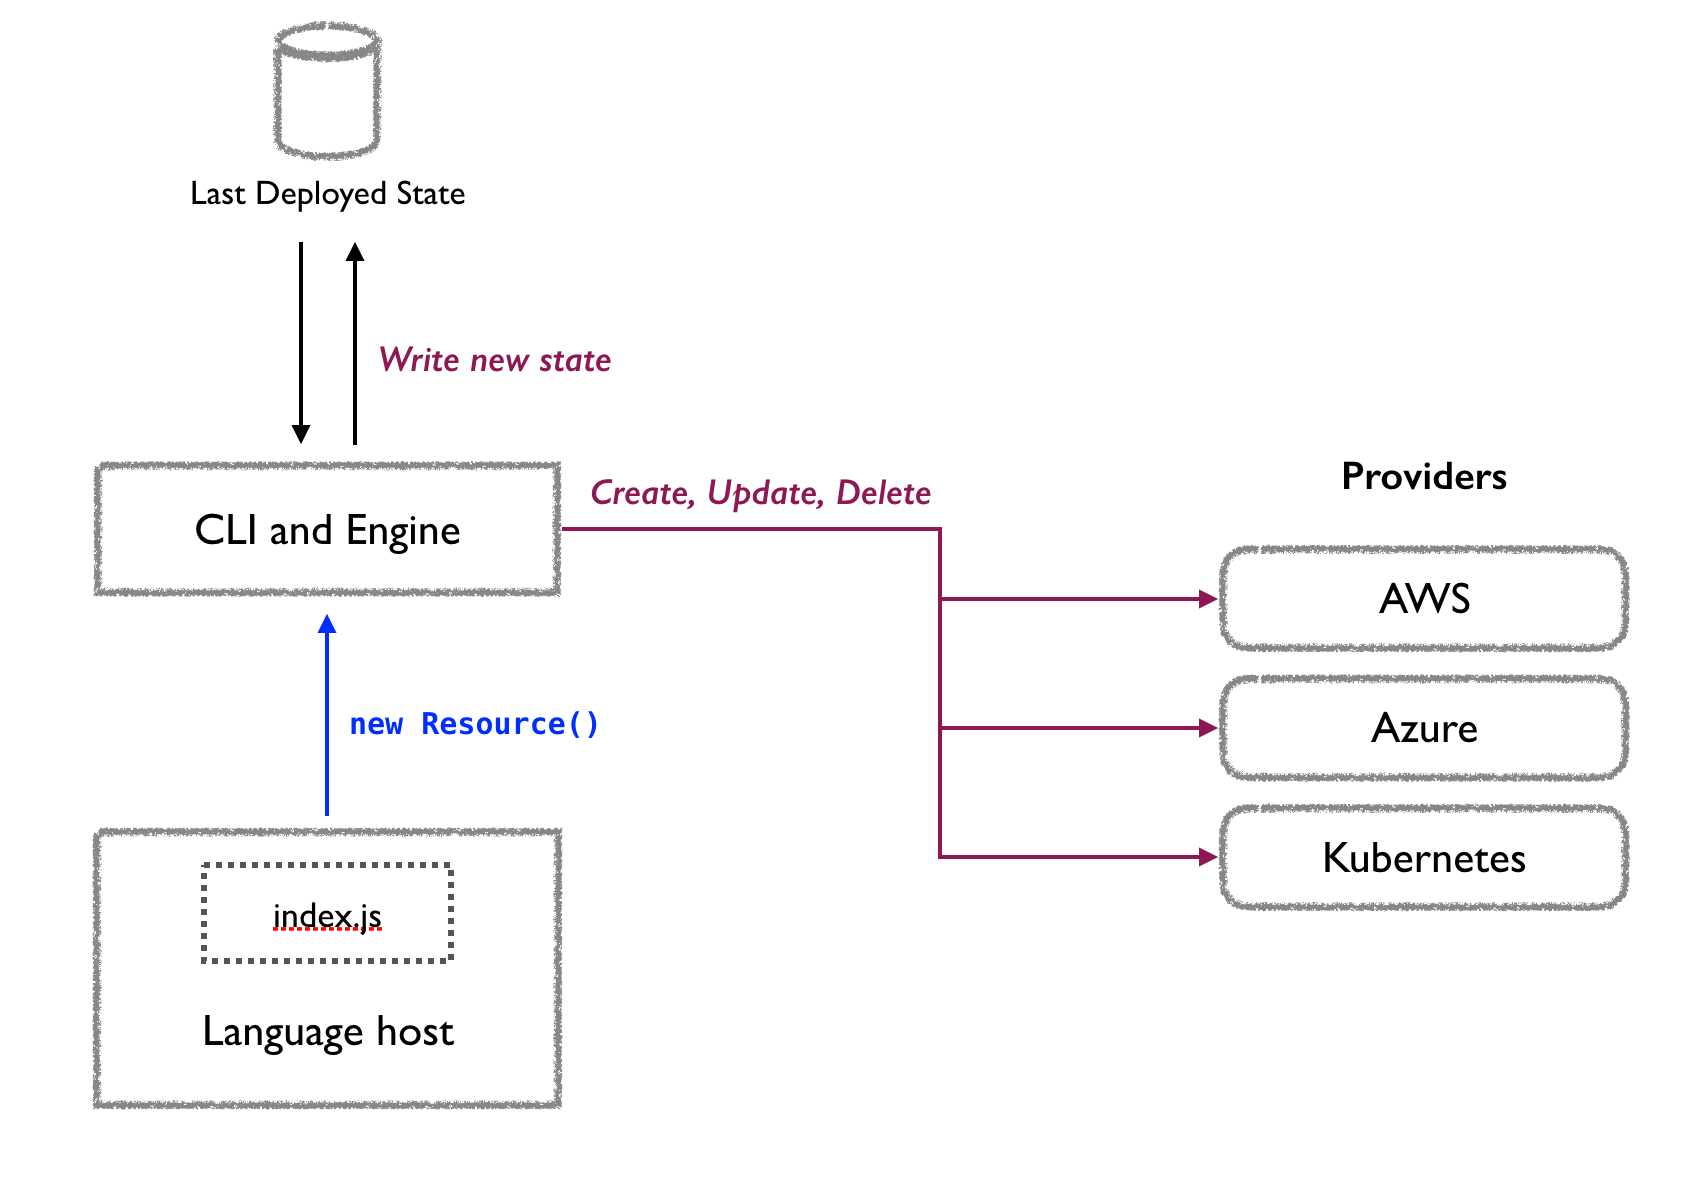
\includegraphics[width=1\columnwidth]{introduction_pulumi/engine-block-diagram} 
  \captionof{figure}{Pulumi architecture}
\end{center}\mbox{}\\
The resources on the cloud providers could drift and their state might get different from the logical description in the state file of the backend engine.
This could happen if an administrator manually modifies the resources without passing through the Pulumi project, or also if the cloud provider changes the APIs on an update.
The \texttt{pulumi refresh} command is telling the engine to check if the states on the cloud providers are corresponding to the logical representation of the state file.
If it is not the case, the resources are modified in order to be aligned with the state file.


\subsection{Pulumi project}
The interesting part for the user is the Pulumi project.
Such a project, that can be created with the \texttt{pulumi new} command, can be any folder that contains a Pulumi.yaml file.
This file specifies the runtime to be used (nodejs, pyhton, Java, etc.) and where to look for the program that should be executed during deployments.\\
The execution of the program will, through the Pulumi APIs, call the Pulumi engine to create the desired resources on the respective cloud providers.

\subsection{The stack}
When creating a new Pulumi application, the first step is to define a \textit{stack}.
A \textit{stack} represents a set of cloud resources that can be managed as a cohesive unit.\\
Each \textit{stack} is associated with an environment.
Tipically, we have a stack for the develop, one for the stage and one for the production.
This is granting us the chance test safely our infrastructure before pushing the changes on production.\\
The \textit{stack} definition typically includes information such as the provider, the region in which the resources should be created, and any required configuration settings.
This information is used by Pulumi to provision and manage the resources in the \textit{stack}.

\subsection{APIs to define the resources to be created}
Once the \textit{stack} is defined, you write code that implements the resource management logic.
Pulumi provides libraries for several programming languages, including TypeScript, Python, Go, .NET, and partially Java.
You use these libraries to create and configure cloud resources.\\
In Pulumi, you define resources using the respective resource constructor functions.
This function takes in the configuration for the resource as input, and returns a reference to the resource to be created.\\
%This reference can then be used to manage the resource throughout its lifecycle.\\
Pulumi code can also contain logic for managing relationships between resources.
For example, you can specify that one resource depends on another, so that Pulumi knows to create the dependent resource first.
Anyway, Pulumi's backend already knows the dependencies between the resources to be created, so in any case he will manage to reorder their creation in a proper way.

\subsection{Creating and updating resources with Pulumi commands}
Once the code is written, you use Pulumi to create the cloud resources specified in the \textit{stack} definition.
Pulumi uses the cloud provider exposed REST APIs to create the resources and their corresponding configurations. 
%The resource creation process is declarative, which means that Pulumi automatically figures out the order in which resources should be created based on their dependencies.\\
%Pulumi also supports continuous delivery, meaning that changes to your code are automatically detected and used to update existing resources.
When a change is detected, Pulumi compares the desired state (based on your code) to the current state (based on the resources in the cloud) and makes any necessary changes to bring the resources into compliance with the desired state.
As we mentioned before, this feature is achieved through the state file that the backend owns.

\subsection{Viewing resources state}
Pulumi provides a command to view the state of the resources managed by the application: \texttt{pulumi stack}.
This command shows the created resources, their properties, and their current state. 
This information can be used to debug issues and ensure that resources are configured correctly.\\
The state of a resource is maintained by Pulumi in a "state file".
This file contains information about the resources that have been created, as well as their current configuration and state.
The state file is automatically updated by Pulumi as resources are created, updated, or deleted.

\subsection{Restoring resources state}
In case of issues or errors during resource creation or management, you can use Pulumi to restore the resource state to the last known good state.
This ensures that cloud resources are always consistent with the code and \textit{stack} definition.\\
Pulumi uses the state file to track the current state of the resources it manages.
If the state of a resource becomes inconsistent with the desired state (for example, if a resource is accidentally deleted), you can use Pulumi to recreate the resource based on the information in the state file.
This restores the resource to its last known good state and brings it back into compliance with the \textit{stack} definition.

\section{Pulumi's Output}
In an IaC context, and therefore with Pulumi, the creation of the resources is not immediate.
Hence, in our code when we call a constructor for a certain resource, we are not actually creating it in that exact moment, but we are rather requesting Pulumi to instantiate such a resource on the given cloud provider.
So, the usage of that resource is not available until Pulumi will have completed its creation on the cloud provider.
How can we perform operations on a resource when we do not know when it will become available?
Pulumi addresses such a problem with the \texttt{Output} type.\\
In Pulumi, \texttt{Output} values are typically computed asynchronously, so that they can represent resources that are being provisioned by cloud providers.
Like a Future in Java, or a Promise in TypeScript, an \texttt{Output} can be used to chain operations that depend on the completion of other operations.
This feature will come handy to chain the definition of resources that depends on other resources.\\
We'll see how to create a Monad out of the \texttt{Output} type so that we'll be able to boost our \textit{syntactic sugar} in the Scala version of the case study.
